% CREATED BY DAVID FRISK, 2016
\chapter{XQBGPPPU Instruction Listing}

\section*{\texttt{max}}

	\begin{wrapfigure}{r}{0.48\textwidth}
		\begin{flushright}
			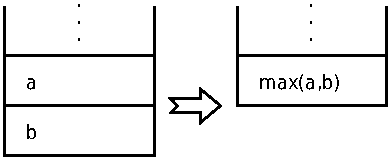
\includegraphics[width=0.9\linewidth]{figure/pdf/i_max} 
		\end{flushright}
	\end{wrapfigure}

		\texttt{max} maxtiplies two fixed-point values on the stack, and stores
		the result on the stack.

\section*{\texttt{min}}

	\begin{wrapfigure}{r}{0.48\textwidth}
		\begin{flushright}
			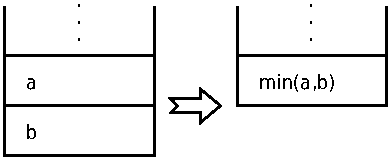
\includegraphics[width=0.9\linewidth]{figure/pdf/i_min} 
		\end{flushright}
	\end{wrapfigure}

		\texttt{min} mintiplies two fixed-point values on the stack, and stores
		the result on the stack.

\section*{\texttt{add}}

	\begin{wrapfigure}{r}{0.48\textwidth}
		\begin{flushright}
			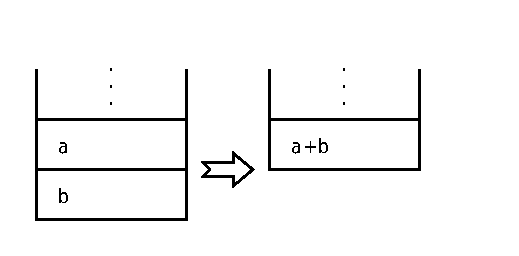
\includegraphics[width=0.9\linewidth]{figure/pdf/i_add} 
		\end{flushright}
	\end{wrapfigure}

		\texttt{add} addtiplies two fixed-point values on the stack, and stores
		the result on the stack.

\section*{\texttt{sub}}

	\begin{wrapfigure}{r}{0.48\textwidth}
		\begin{flushright}
			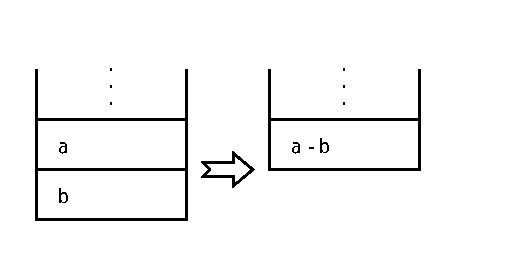
\includegraphics[width=0.9\linewidth]{figure/pdf/i_sub} 
		\end{flushright}
	\end{wrapfigure}

		\texttt{sub} subtiplies two fixed-point values on the stack, and stores
		the result on the stack.

\section*{\texttt{mul}}

	\begin{wrapfigure}{r}{0.48\textwidth}
		\begin{flushright}
			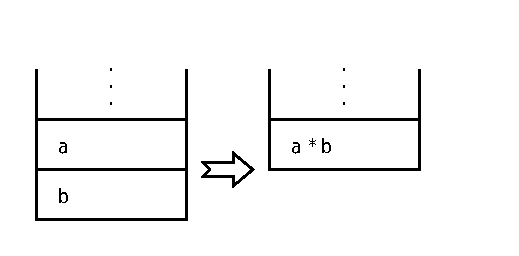
\includegraphics[width=0.9\linewidth]{figure/pdf/i_mul} 
		\end{flushright}
	\end{wrapfigure}

		\texttt{mul} multiplies two fixed-point values on the stack, and stores
		the result on the stack.

\section*{\texttt{div}}

	\begin{wrapfigure}{r}{0.48\textwidth}
		\begin{flushright}
			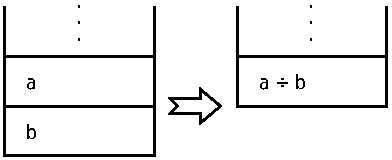
\includegraphics[width=0.9\linewidth]{figure/pdf/i_div} 
		\end{flushright}
	\end{wrapfigure}

		\texttt{div} divtiplies two fixed-point values on the stack, and stores
		the result on the stack.

\section*{\texttt{sqrt}}

	\begin{wrapfigure}{r}{0.48\textwidth}
		\begin{flushright}
			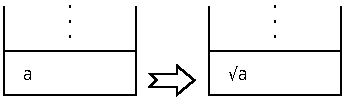
\includegraphics[width=0.9\linewidth]{figure/pdf/i_sqrt} 
		\end{flushright}
	\end{wrapfigure}

		\texttt{sqrt} sqrttiplies two fixed-point values on the stack, and stores
		the result on the stack.

\section*{\texttt{abs}}

	\begin{wrapfigure}{r}{0.48\textwidth}
		\begin{flushright}
			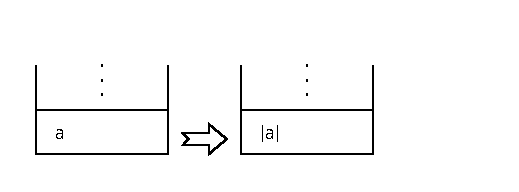
\includegraphics[width=0.9\linewidth]{figure/pdf/i_abs} 
		\end{flushright}
	\end{wrapfigure}

		\texttt{abs} abstiplies two fixed-point values on the stack, and stores
		the result on the stack.

\section*{\texttt{floor}}

	\begin{wrapfigure}{r}{0.48\textwidth}
		\begin{flushright}
			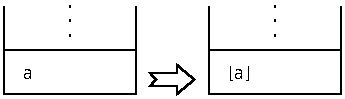
\includegraphics[width=0.9\linewidth]{figure/pdf/i_floor} 
		\end{flushright}
	\end{wrapfigure}

		\texttt{floor} floortiplies two fixed-point values on the stack, and stores
		the result on the stack.

\section*{\texttt{acc}}

	\begin{wrapfigure}{r}{0.48\textwidth}
		\begin{flushright}
			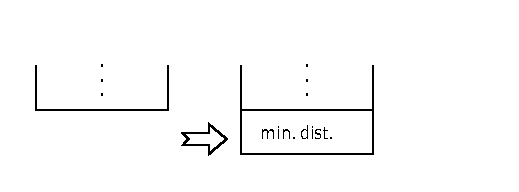
\includegraphics[width=0.9\linewidth]{figure/pdf/i_acc} 
		\end{flushright}
	\end{wrapfigure}

		\texttt{acc} acctiplies two fixed-point values on the stack, and stores
		the result on the stack.

\section*{\texttt{dot}}

	\begin{wrapfigure}{r}{0.48\textwidth}
		\begin{flushright}
			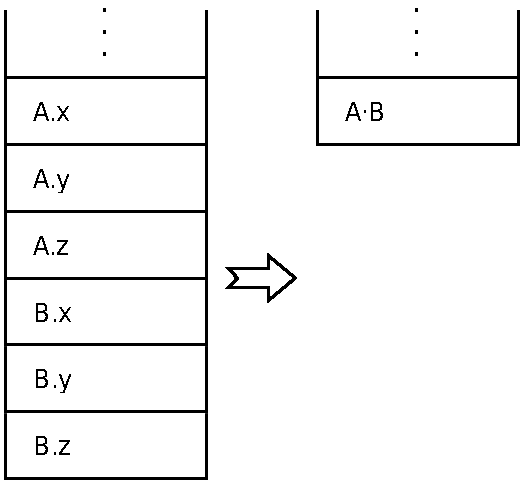
\includegraphics[width=0.9\linewidth]{figure/pdf/i_dot} 
		\end{flushright}
	\end{wrapfigure}

		\texttt{dot} dottiplies two fixed-point values on the stack, and stores
		the result on the stack.

\section*{\texttt{cross}}

	\begin{wrapfigure}{r}{0.48\textwidth}
		\begin{flushright}
			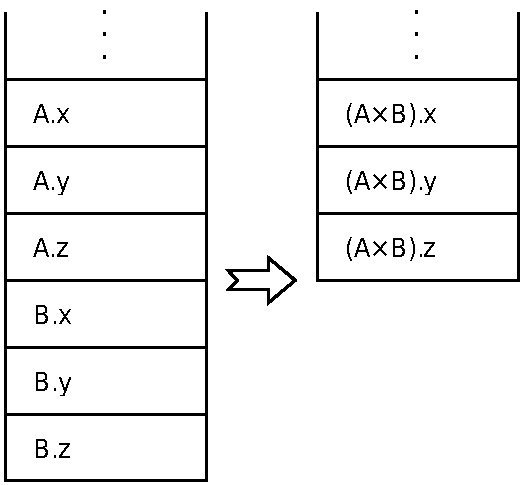
\includegraphics[width=0.9\linewidth]{figure/pdf/i_cross} 
		\end{flushright}
	\end{wrapfigure}

		\texttt{cross} crosstiplies two fixed-point values on the stack, and stores
		the result on the stack.

\section*{\texttt{addv}}

	\begin{wrapfigure}{r}{0.48\textwidth}
		\begin{flushright}
			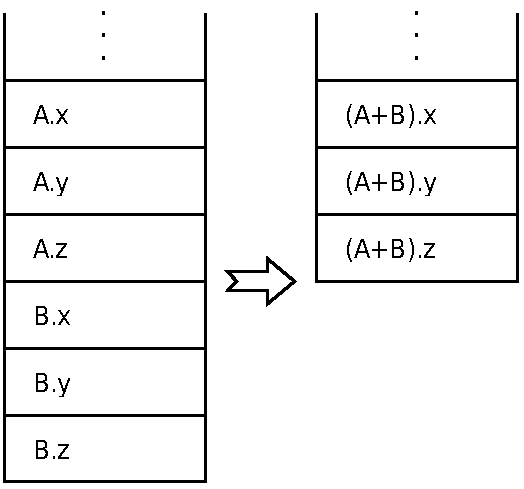
\includegraphics[width=0.9\linewidth]{figure/pdf/i_addv} 
		\end{flushright}
	\end{wrapfigure}

		\texttt{addv} addvtiplies two fixed-point values on the stack, and stores
		the result on the stack.

\section*{\texttt{subv}}

	\begin{wrapfigure}{r}{0.48\textwidth}
		\begin{flushright}
			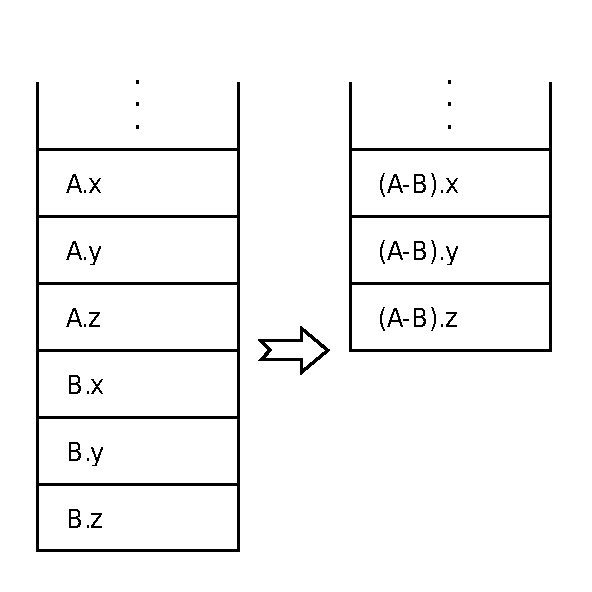
\includegraphics[width=0.9\linewidth]{figure/pdf/i_subv} 
		\end{flushright}
	\end{wrapfigure}

		\texttt{subv} subvtiplies two fixed-point values on the stack, and stores
		the result on the stack.

\section*{\texttt{scale}}

	\begin{wrapfigure}{r}{0.48\textwidth}
		\begin{flushright}
			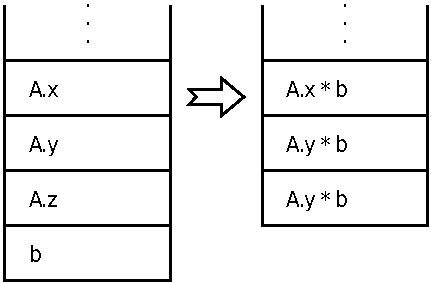
\includegraphics[width=0.9\linewidth]{figure/pdf/i_scale} 
		\end{flushright}
	\end{wrapfigure}

		\texttt{scale} scaletiplies two fixed-point values on the stack, and stores
		the result on the stack.

\section*{\texttt{copy}}

	\begin{wrapfigure}{r}{0.48\textwidth}
		\begin{flushright}
			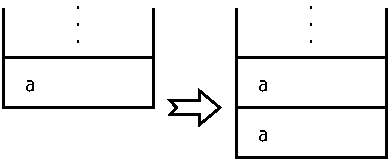
\includegraphics[width=0.9\linewidth]{figure/pdf/i_copy} 
		\end{flushright}
	\end{wrapfigure}

		\texttt{copy} copytiplies two fixed-point values on the stack, and stores
		the result on the stack.

\section*{\texttt{swap}}

	\begin{wrapfigure}{r}{0.48\textwidth}
		\begin{flushright}
			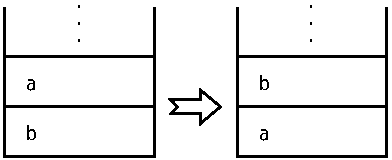
\includegraphics[width=0.9\linewidth]{figure/pdf/i_swap} 
		\end{flushright}
	\end{wrapfigure}

		\texttt{swap} swaptiplies two fixed-point values on the stack, and stores
		the result on the stack.
